% --------------------------------------
% Document Class
% --------------------------------------
\documentclass[a4paper,11pt]{article}
% --------------------------------------



% --------------------------------------
% Use Package
% --------------------------------------


\usepackage[francais]{babel}
%\usepackage{ucs}
\usepackage[utf8]{inputenc}
\usepackage[T1]{fontenc}

\usepackage{makeidx}
\usepackage{color}
\usepackage{graphicx}
\usepackage{float}
\usepackage[hidelinks]{hyperref} 
\usepackage{geometry}
%\usepackage{lastpage}
%\usepackage{marginnote}
\usepackage{fancyhdr}
%\usepackage{titlesec}
%\usepackage{framed}
\usepackage{amsmath}
\usepackage{empheq}
\usepackage{array}
\usepackage{multicol}
%\usepackage{adjustbox}

% insert code
\usepackage{listings}

% define our color
\usepackage{xcolor}

% code color
\definecolor{ligthyellow}{RGB}{250,247,220}
\definecolor{darkblue}{RGB}{5,10,85}
\definecolor{ligthblue}{RGB}{1,147,128}
\definecolor{darkgreen}{RGB}{8,120,51}
\definecolor{darkred}{RGB}{160,0,0}

% other color
\definecolor{ivi}{RGB}{141,107,185}


\lstset{
    language=Scilab,
    captionpos=b,
    extendedchars=true,
    frame=lines,
    numbers=left,
    numberstyle=\tiny,
    numbersep=5pt,
    keepspaces=true,
    breaklines=true,
    showspaces=false,
    showstringspaces=false,
    breakatwhitespace=false,
    stepnumber=1,
    showtabs=false,
    tabsize=3,
    basicstyle=\small\ttfamily,
    backgroundcolor=\color{ligthyellow},
    keywordstyle=\color{ligthblue},
    morekeywords={include, printf, uchar},
    identifierstyle=\color{darkblue},
    commentstyle=\color{darkgreen},
    stringstyle=\color{darkred},
}


% --------------------------------------



% --------------------------------------
% Page setting
% --------------------------------------
%\pagestyle{empty}
\setlength{\headheight}{15pt}

\setcounter{secnumdepth}{3}
\setcounter{tocdepth}{2}

\makeatletter
\@addtoreset{chapter}{part}
\makeatother 

\hypersetup{         % parametrage des hyperliens
  colorlinks=true,      % colorise les liens
  breaklinks=true,      % permet les retours à la ligne pour les liens trop longs
  urlcolor= blue,       % couleur des hyperliens
  linkcolor= black,     % couleur des liens internes aux documents (index, figures, tableaux, equations,...)
  citecolor= green      % couleur des liens vers les references bibliographiques
}

% --------------------------------------

% --------------------------------------
% Information
% --------------------------------------
\title{Compte-rendu TP2 TI : Projection perspective}
\author{Elliot VANEGUE et Gaëtan DEFLANDRE}
% --------------------------------------

\definecolor{myColor}{rgb}{0.5, 0.1, 0.75}

% --------------------------------------
% Begin content
% --------------------------------------
\begin{document}

% Set language to english
  \selectlanguage{francais}

  % Start the page counting
  \pagenumbering{arabic}

  \maketitle
  
  \mbox{}
  \newpage
  \clearpage
  
  \section*{Introduction}
  Lors de ce TP, nous allons voir les différentes étapes permettant de passer d'un
  modèle 3D à sa projection bidimensionnelle. Pour cela nous avons besoin de calculer les matrices 
  extrinsèque et intrinsèque qui vont nous permettre de déterminer les coordonnées des points
  sur un plan 2D, d'un objet 3D au départ.
  
  \section{Modèles d'objets 3D et affichage 2D}
  Dans un premier temps nous allons faire varier les paramètres présents dans l'exemple fournit
  dans le cadre de ce TP, afin d'observer la variation des coordonnées des points de la projection de l'objet.\\
  
  \begin{figure}[H]
    \center
    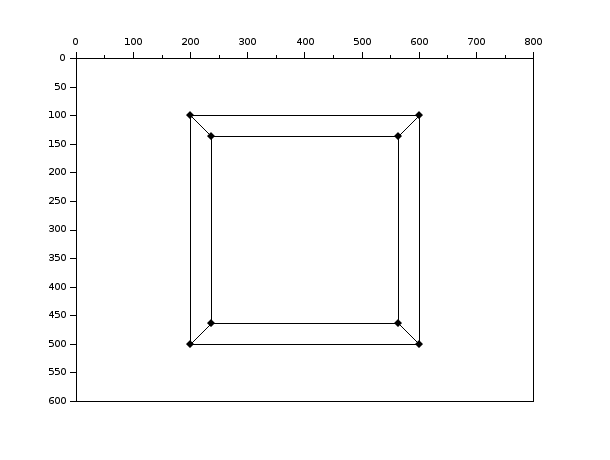
\includegraphics[width=10cm]{Projection1.png}
    \caption{Image du cube avec la matrice de projection de base}
  \end{figure}

  
  Au départ, nous avons une matrice de projection qui vaut : 
  $\begin{pmatrix}
   -360 & 0 & 80 & 400 \\
   0 & -360 & 60 & 300 \\
   0 & 0 & 0.2 & 1
  \end{pmatrix}$
  Nous avons constaté que si nous modifions les valeurs -360, la largeur et la hauteur de la représentation du cube sont modifiés.
  Lorsque nous modifions les valeurs 80 ou 60, on remarque que le point de vue du capteur est légèrement décalé, car nous pouvons 
  voir une des faces latérales sur l'image résultante. Et si nous modifions les valeurs 400 ou 300, nous observons que c'est l'objet qui translate.\\
  
  \begin{figure}[H]
    \center
    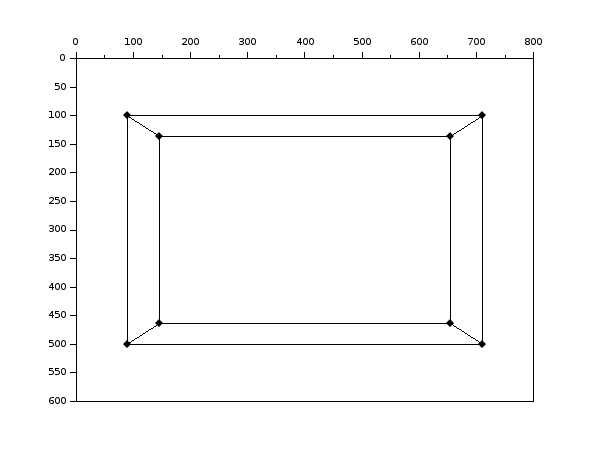
\includegraphics[width=5cm]{ProjectionTaille.png}
    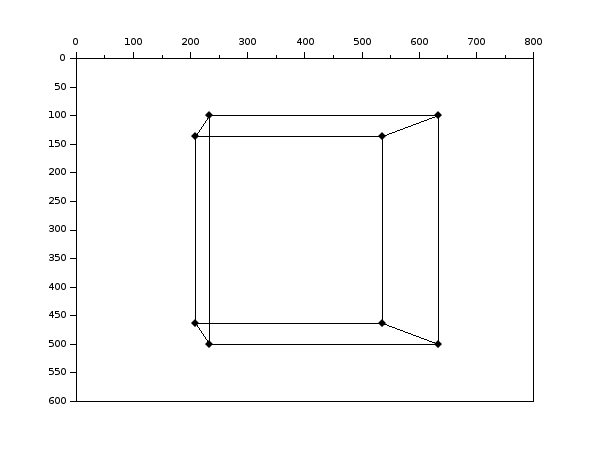
\includegraphics[width=5cm]{ProjectionRotation.png}
    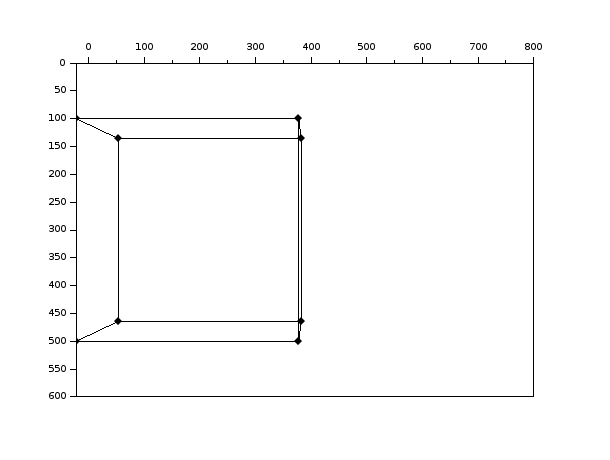
\includegraphics[width=5cm]{ProjectionTranslation.png}
    \caption{Image du cube avec différentes modifiction sur la matrice de projection}
  \end{figure}
  
  Nous avons ensuite modifié ces paramètres sur une grille 2D. Nous remarquons que les modifications apportées à la 
  matrice de projection ont le même effet pour cette forme.
  Cependant, la translation du capteur ne modifie pas l'image, car cette forme n'a pas de profondeur et donc aucune autre face n'est affichable.
  
  \section{Matrice extrinsèque}
  
  Nous allons maintenant chercher à calculer la matrice extrinsèque. Cette matrice prend en compte des paramètres qui dépendent de la position 
  de la caméra dans l'environnement, comme la rotation ou la translation effectuée par la caméra. Pour calculer cette matrice, nous l'avons 
  décomposé en plusieurs sous-matrices que nous devrons multiplier. Voici les matrices composant la matrice extrinsèque :\\
  
  \begin{itemize}
   \item matrice de rotation x : 
   $\begin{pmatrix}
     1 & 0 & 0\\
     0 & cos(theta) & -sin(theta)\\
     0 & sin(theta) & cos(theta)
    \end{pmatrix}$
    
   \item matrice de rotation y : 
   $\begin{pmatrix}
     cos(theta) & 0 & sin(theta)\\
     0 & 1 & 0\\
     -sin(theta) & 0 & cos(theta)
    \end{pmatrix}$
    
   \item matrice de rotation z : 
   $\begin{pmatrix}
     cos(theta) & -sin(theta) & 0\\
     sin(theta) & cos(theta) & 0\\
     0 & 0 & 1
    \end{pmatrix}$
    
   \item matrice de translation : 
   $\begin{pmatrix}
     x\\
     y\\
     z
    \end{pmatrix}$

  \end{itemize}
  
  Une fois ces matrices définient, nous les multiplions afin d'obtenir la matrice
  extrinsèque qui a la forme suivante :\\
  \begin{center}
    $\begin{pmatrix}
      R_{x/x} & R_{x/y} & R_{x/z} & t_{x}\\
      R_{y/x} & R_{y/y} & R_{y/z} & t_{y}\\
      R_{z/x} & R_{z/y} & R_{z/z} & t_{z}\\
      0 & 0 & 0 & 1
      \end{pmatrix}$
  \end{center}
  
  Nous avons ensuite calculé les matrices extrinsèques de deux exemples du TP.\\
  
  \begin{itemize}
   \item E1 : Cette exemple place la caméra en dessous du cube. Pour cela il suffit
   d'effectué une translation de la caméra sur l'axe \textit{z}. 
  
   Ce qui nous donne le résultat de la matrice extrinsèque suivant :
    $\begin{pmatrix}
      1 & 0 & 0 & 0\\
      0 & 1 & 0 & 0\\
      0 & 0 & 1 & 5\\
      0 & 0 & 0 & 1
      \end{pmatrix}$.
   \item E2 : Dans cette exemple la caméra se positionne à 5m sur la diagonale principale.
   La caméra regarde donc un des coins supérieur du cube. Pour cela il faut que la caméra 
   fasse une rotation sur \textit{y} de 45\degre pour que la caméra regarde une des arêtes du cube. Puis,
   il faut faire une rotation de 45\degre sur l'axe \textit{z} pour se positionner dans le coin du cube. 
   Et enfin, effectué une translation de 5m sur la caméra sur l'axe \textit{x}. Le résultat donne la matrice
   $\begin{pmatrix}
      0.7 & 0 & 0.7 & 0\\
      0.5 & 0.7 & -0.5 & 0\\
      -0.5 & 0.7 & 0.5 & -5\\
      0 & 0 & 0 & 1
      \end{pmatrix}$.
  \end{itemize}
  
  % TODO avoir si les résultat actuel fonctionne toujours à la fin du TP
  
  \section{Matrice intrinsèque}
  
  Nous allons maintenant calculer la matrice intrinsèque qui dépend de paramètres propres à la caméra comme sa 
  distance focale, les facteurs d'agrandissement de l'image... Pour cela nous devons d'abord passer par une matrice 
  de projection, puis de changement de repère. Nous allons calculer ces matrices à partir des données fournies dans le TP.\\
  
  matrice de projection : 
   $\begin{pmatrix}
     f & 0 & 0\\  
     0 & f & 0\\  
     0 & 0 & 1 
     \end{pmatrix}$ = 
   $\begin{pmatrix}
     20 & 0 & 0\\  
     0 & 20 & 0\\  
     0 & 0 & 1 
     \end{pmatrix}$\\
     
  matrice de changement de repère : 
   $\begin{pmatrix}
     1/s_x & 0 & 0\\  
     0 & 1/s_y & 0\\  
     0 & 0 & 1 
     \end{pmatrix}$ = 
   $\begin{pmatrix}
     0.011 & 0 & 0\\  
     0 & 0.007875 & 0\\  
     0 & 0 & 1 
     \end{pmatrix}$\\
     
  A partir de ces deux matrices, nous pouvons calculer la matrice intrinsèque en les multipliants.
  Une fois, la matrice intrinsèque formé, nous allons diviser la matrice par la coordonnée \textit{z},
  ce qui nous donnera une matrice à deux dimensions. La troisième dimension valant 1, celle-ci ne sera
  plus utilisé.
     
  \section{Projection et affichage des objets}
  
  
  \section*{Conclusion}
  Nous avons pu voir grâce à ce TP, qu'il est possible de passer d'un repère trois dimension à un repère deux
  dimension grâce à un ensemble de paramètres réuni dans deux matrices.
    
\end{document}